\documentclass[a4paper,10pt]{article}

\usepackage[T1]{fontenc}
\usepackage{lmodern}
\usepackage{graphicx}
\usepackage{fancyhdr}
\usepackage{geometry}
\usepackage{amsmath}
\usepackage{float} % For positioning images
\usepackage{subcaption} % For subfigures
\usepackage{booktabs}
\usepackage{tabularx}
\usepackage{enumitem}
\usepackage{tikz}
\usetikzlibrary{shapes,arrows.meta,positioning,fit,backgrounds,calc}

% Page Geometry
\geometry{a4paper, total={170mm,257mm}, left=20mm, right=20mm, top=30mm, bottom=30mm, headheight=52pt}

% Page Header/Footer Setup
\pagestyle{fancy}
\fancyhf{}
\fancyhead[L]{
\includegraphics[width=2cm]{intermediate_files/iiitb_logo.jpg}}
\fancyfoot[L]{International Institute of Information Technology, Bangalore}
\fancyfoot[R]{Page \thepage}

\setlist{itemsep=1pt, topsep=3pt}
\newcommand{\code}[1]{\texttt{\detokenize{#1}}}
\newcolumntype{Y}{>{\raggedright\arraybackslash}X}

% Title Details
\title{\Large\textbf{S.P.D. Emergency: A Distributed Emergency Resource Matching System} \\
    \normalsize Project Report \\
    \normalsize Chaitya Nirmal Shah (IMT2023055) \\
    \normalsize Velidanda Krishna Sai (IMT2023094) \\[6pt]
    \normalsize Repository: \texttt{github.com/CShah44/spd-emergency} \\
    \normalsize Branch to look at: \texttt{main} \\
    }
\date{}

\begin{document}

\maketitle
\thispagestyle{fancy}

%--------------------------------------------------------------------
\section{Introduction}

This project is a system that connects people who need emergency help with people or
organisations who can give it. Someone affected by a flood can post a request for drinking
water. The owner of a water tanker can register the tanker as a resource. The system finds the
nearest available resource of the right type and assigns it to the request. A request can be for
water, food, medicine, transport or shelter.

The system is made of a request service that clients talk to, a RabbitMQ message broker, a
matching service, a coordinator, and six storage nodes arranged as three shards with one replica
each. Every service runs in a Docker container, and the whole system is deployed on Kubernetes.
Around this core are metrics and a dashboard, load and failure tests, sharding by location,
autoscaling of the matching service, a second coordinator, and a log-based way for a storage node
to catch up after it has been down.

The services are written in Python 3.12 with FastAPI. The web page is written in Svelte. The rest
is existing software: RabbitMQ, SQLite, Prometheus, Grafana, KEDA, Docker and Kubernetes. This
report describes what each part does, how it is built, and the measurements taken on it.

%--------------------------------------------------------------------
\section{System Overview}

The system has three layers.
\begin{itemize}
    \item \textbf{Application layer.} The request service takes requests from clients, RabbitMQ
    holds the work that is waiting, and the matching service does the matching. A web page and a
    command-line client sit on top.
    \item \textbf{Storage layer.} A coordinator decides where each record lives. Six storage nodes
    hold the records: three shards, each with a primary and a replica.
    \item \textbf{Platform layer.} Every service runs in a Docker container. Docker Compose runs
    them on one machine and Kubernetes runs them as a cluster. KEDA scales the matching service,
    and Prometheus and Grafana show what is happening.
\end{itemize}

\subsection*{One request from start to end}
\begin{enumerate}
    \item The client sends \code{POST /requests}. The request service checks the input.
    \item The request is saved through the coordinator, which picks the shard and writes to both
    copies.
    \item A small message with the request id is published to RabbitMQ and the client gets
    \code{201} straight away. The client does not wait for matching.
    \item A matching service pod takes the message, finds the nearest free resource of the same
    type within 50~km, claims it, and marks the request \code{MATCHED} (or \code{UNMATCHED} if
    there is none). Then it acknowledges the message.
    \item The client reads the result with \code{GET /requests/{id}}.
\end{enumerate}

\begin{figure}[H]
    \centering
    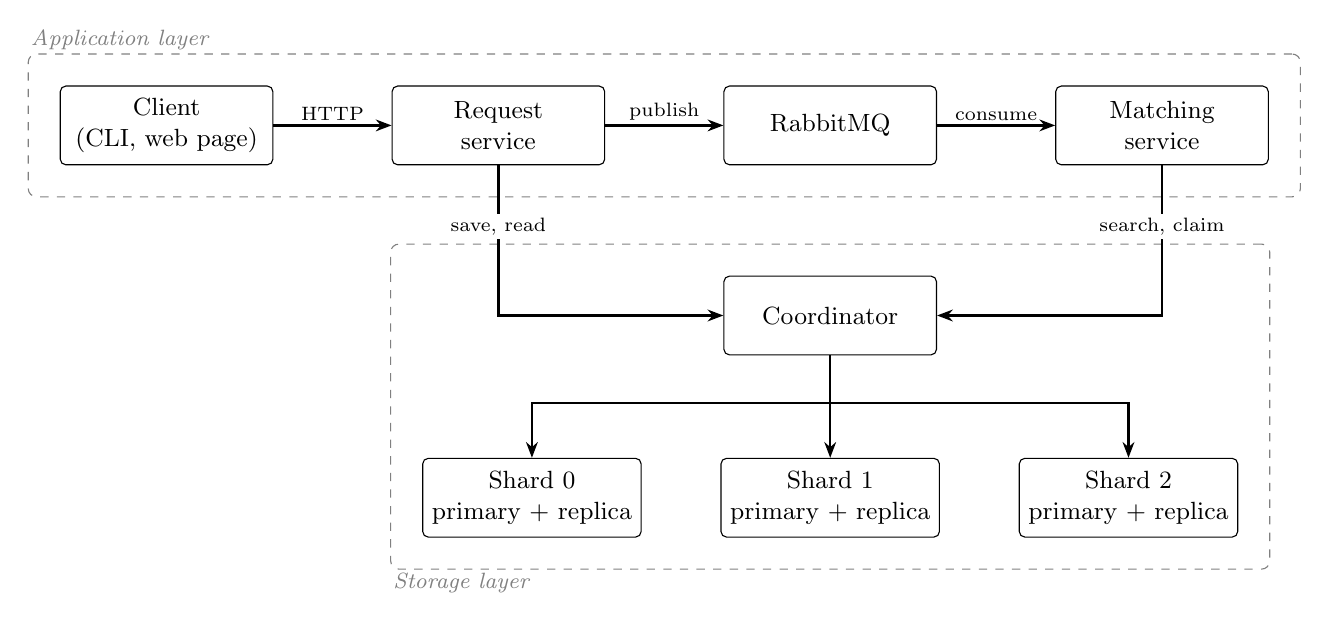
\begin{tikzpicture}[
        box/.style={draw, rounded corners=2pt, minimum width=27mm, minimum height=10mm,
                    align=center, font=\small},
        arr/.style={-{Stealth[length=2mm]}, thick},
        lab/.style={font=\scriptsize, above, inner sep=1.5pt}]

        \node[box] (client) {Client\\(CLI, web page)};
        \node[box, right=15mm of client] (req) {Request\\service};
        \node[box, right=15mm of req] (mq) {RabbitMQ};
        \node[box, right=15mm of mq] (match) {Matching\\service};

        \node[box, below=14mm of mq] (coord) {Coordinator};

        \node[box, below=13mm of coord] (s1) {Shard 1\\primary + replica};
        \node[box, left=10mm of s1] (s0) {Shard 0\\primary + replica};
        \node[box, right=10mm of s1] (s2) {Shard 2\\primary + replica};

        \draw[arr] (client) -- node[lab] {HTTP} (req);
        \draw[arr] (req) -- node[lab] {publish} (mq);
        \draw[arr] (mq) -- node[lab] {consume} (match);

        \draw[arr] (req.south) |- node[lab, pos=0.25, above=0pt, fill=white] {save, read} (coord.west);
        \draw[arr] (match.south) |- node[lab, pos=0.25, above=0pt, fill=white] {search, claim} (coord.east);

        \draw[arr] (coord.south) -- ++(0,-6mm) -| (s0.north);
        \draw[arr] (coord.south) -- (s1.north);
        \draw[arr] (coord.south) -- ++(0,-6mm) -| (s2.north);

        \begin{scope}[on background layer]
            \node[draw=gray, dashed, rounded corners=3pt, fit=(client)(req)(mq)(match),
                  inner sep=4mm] (applayer) {};
            \node[draw=gray, dashed, rounded corners=3pt, fit=(coord)(s0)(s1)(s2),
                  inner sep=4mm] (stlayer) {};
        \end{scope}
        \node[font=\footnotesize\itshape, text=gray, anchor=south west, inner sep=1pt]
            at (applayer.north west) {Application layer};
        \node[font=\footnotesize\itshape, text=gray, anchor=north west, inner sep=1pt]
            at (stlayer.south west) {Storage layer};
    \end{tikzpicture}
    \caption{The main parts of the system. Platform pieces (Kubernetes, KEDA, Prometheus,
    Grafana) are not drawn.}
    \label{fig:arch}
\end{figure}

\begin{table}[H]
    \centering
    \small
    \begin{tabularx}{\textwidth}{l Y Y l}
        \toprule
        Part & What it does & Stack & Count \\
        \midrule
        Request service & Client REST API; validates and stores requests, queues a match message & FastAPI, Uvicorn, pydantic, httpx, pika & 2 pods \\
        RabbitMQ & Holds match work until a matcher is free & RabbitMQ 3.13, AMQP & 1 \\
        Matching service & Takes messages and assigns resources & FastAPI, pika, httpx & 1 to 5 pods \\
        Web page & Live dashboard and demo controls & Svelte 5, Vite, served by FastAPI & 1 \\
        Coordinator & Picks the shard, routes calls, watches heartbeats, handles failover & FastAPI, async httpx & 2 pods, 1 leads \\
        Storage node & Stores versioned records on its own disk & FastAPI, SQLite & 6 \\
        Monitoring & Collects and draws metrics & prometheus-client, Prometheus, Grafana & 1 each \\
        Autoscaler & Sets the number of matching pods & KEDA (RabbitMQ scaler) & 1 \\
        \bottomrule
    \end{tabularx}
    \caption{Components and the stack each one uses.}
    \label{tab:components}
\end{table}

%--------------------------------------------------------------------
\section{Data and Rules}

Requests and resources are stored as JSON with a fixed shape. Matching uses only the fixed
fields (type, location and status). Free text such as the request details is never interpreted.

A \textbf{request} has an id, a type, a location (latitude and longitude), a quantity, free-text
details, a contact, a status, the id of the assigned resource, timestamps, and a version number.
A \textbf{resource} has the same kind of fields plus a name, a capacity and an availability note.
The type is one of \code{water}, \code{food}, \code{medicine}, \code{transport} and
\code{shelter}. Anything else is rejected with \code{400}. Quantity and capacity are stored, but
the matching does not use them yet.

Ids look like \code{req-<cell>-<16 hex characters>}, where the cell is a short code for the area
of the location (see Section~\ref{sec:geo}).

\subsection{Statuses}

A request moves along the path in Figure~\ref{fig:status}. Any other move is refused with
\code{409}. A client can only set \texttt{IN\_PROGRESS}, \code{FULFILLED}, \code{CANCELLED} and
the retry back to \code{PENDING}. Only the matching service sets \code{MATCHED} and
\code{UNMATCHED}, because only it knows whether a resource was really assigned.

A resource is \code{AVAILABLE}, \code{ASSIGNED} or \code{OFFLINE}. It goes back from
\code{ASSIGNED} to \code{AVAILABLE} when its request is fulfilled or cancelled. It cannot go
straight from \code{ASSIGNED} to \code{OFFLINE}, so a request is never left without its helper.

\begin{figure}[htbp]
    \centering
    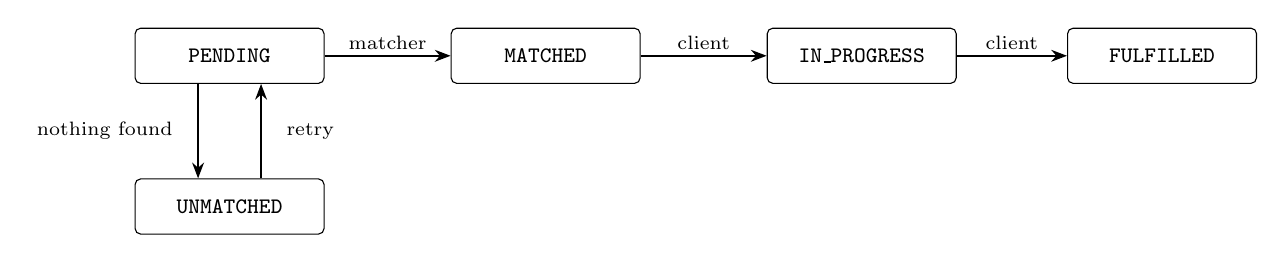
\begin{tikzpicture}[
        st/.style={draw, rounded corners=2pt, minimum width=24mm, minimum height=7mm,
                   font=\footnotesize\ttfamily, align=center},
        arr/.style={-{Stealth[length=2mm]}, thick},
        lab/.style={font=\scriptsize, above, inner sep=2pt}]

        \node[st] (p) {PENDING};
        \node[st, right=16mm of p] (m) {MATCHED};
        \node[st, right=16mm of m] (i) {IN\_PROGRESS};
        \node[st, right=14mm of i] (f) {FULFILLED};
        \node[st, below=12mm of p] (u) {UNMATCHED};

        \draw[arr] (p) -- node[lab] {matcher} (m);
        \draw[arr] (m) -- node[lab] {client} (i);
        \draw[arr] (i) -- node[lab] {client} (f);
        \draw[arr] ([xshift=-4mm]p.south) -- ([xshift=-4mm]u.north);
        \draw[arr] ([xshift=4mm]u.north) -- ([xshift=4mm]p.south);
        \node[font=\scriptsize, anchor=west] at ([xshift=6mm]$(p.south)!0.5!(u.north)$) {retry};
        \node[font=\scriptsize, anchor=east] at ([xshift=-6mm]$(p.south)!0.5!(u.north)$) {nothing found};
    \end{tikzpicture}
    \caption{Life of a request. Arrows are labelled with who makes the move. A request can also
    be set to \texttt{CANCELLED} from any state except \texttt{FULFILLED}.}
    \label{fig:status}
\end{figure}

\subsection{Version numbers}

Every record has a version that goes up by one on every change. A write can say ``save this only
if the version is still $N$''. If someone else changed the record first, the write is refused
with \code{409}. This is how the system avoids giving one resource to two requests
(Section~\ref{sec:matcher}). It does not use locks, so it also works when several matchers run
on different machines.

%--------------------------------------------------------------------
\section{Application Layer}

\subsection{Request service}

This is the only service a client talks to. It validates the input, saves records through the
coordinator, and queues the matching work. Table~\ref{tab:api} lists its API.

\begin{table}[htbp]
    \centering
    \small
    \begin{tabularx}{\textwidth}{l l Y}
        \toprule
        Method and path & Success & Purpose \\
        \midrule
        \code{POST /requests} & 201 & Create a request \\
        \code{GET /requests/{id}} & 200 & Read a request \\
        \code{PUT /requests/{id}/status} & 200 & Move a request along its life cycle \\
        \code{POST /resources} & 201 & Register a resource \\
        \texttt{GET /resources?type=\&status=} & 200 & List resources \\
        \code{PUT /resources/{id}/status} & 200 & Set a resource \code{AVAILABLE} or \code{OFFLINE} \\
        \code{POST /match/{id}} & 200 & Match a request now instead of waiting for the queue \\
        \bottomrule
    \end{tabularx}
    \caption{Client REST API. Errors: invalid input is 400, unknown id 404, illegal status
    move 409, storage unavailable 503.}
    \label{tab:api}
\end{table}

The request is saved before it is queued, and the message is published with publisher confirms.
If RabbitMQ is down at that moment, the request stays saved as \code{PENDING} and the client still
gets \code{201}. The matching service picks it up later (Section~\ref{sec:matcher}).

\subsection{RabbitMQ}

RabbitMQ carries one small message per request: \texttt{\{"request\_id": ..., "attempt": 1\}}. The
setup is a direct exchange called \code{emergency} and a durable queue called
\code{match.requests}, with persistent messages. In Kubernetes it runs as a StatefulSet with its own
disk, so queued messages survive a restart of the broker.

The matching service reads one message at a time and acknowledges it only after the request has
been marked \code{MATCHED} or \code{UNMATCHED}. If a pod dies in the middle of a job, RabbitMQ gives
the message to another pod. A message that fails three times goes to a dead-letter queue
(\code{match.requests.dlq}) instead of being retried forever. A storage outage does not use up an
attempt, since it is not the message's fault.

\subsection{Matching service}
\label{sec:matcher}

The matching service runs a consumer thread that reads the queue, and also answers
\code{POST /match/{id}} for matching on demand. The steps for one request are in
Figure~\ref{fig:match}.

\begin{figure}[htbp]
    \centering
    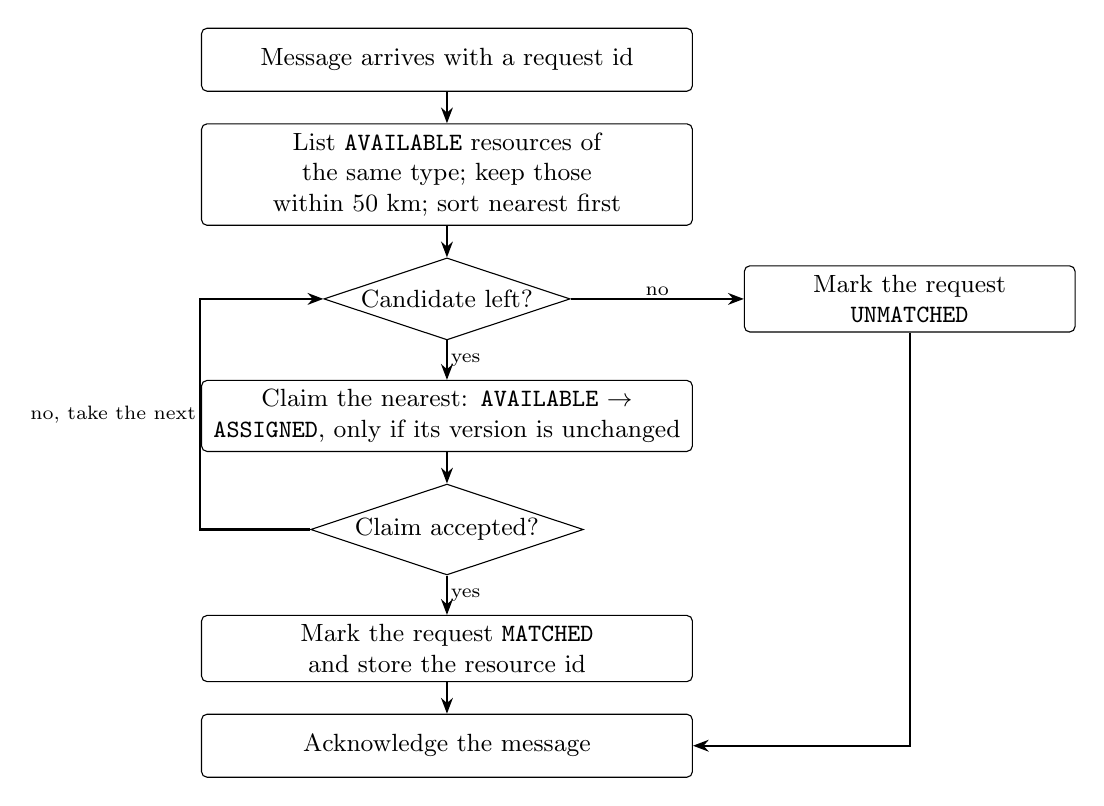
\begin{tikzpicture}[
        box/.style={draw, rounded corners=2pt, minimum width=62mm, minimum height=8mm,
                    align=center, font=\small, text width=60mm},
        dec/.style={draw, diamond, aspect=3, inner sep=1pt, align=center, font=\small},
        arr/.style={-{Stealth[length=2mm]}, thick},
        lab/.style={font=\scriptsize, inner sep=1pt}]

        \node[box] (a) {Message arrives with a request id};
        \node[box, below=4mm of a] (b) {List \texttt{AVAILABLE} resources of the same type; keep
            those within 50~km; sort nearest first};
        \node[dec, below=4mm of b] (c) {Candidate left?};
        \node[box, below=5mm of c] (d) {Claim the nearest: \texttt{AVAILABLE} $\to$ \texttt{ASSIGNED},
            only if its version is unchanged};
        \node[dec, below=4mm of d] (e) {Claim accepted?};
        \node[box, below=5mm of e] (f) {Mark the request \texttt{MATCHED} and store the resource id};
        \node[box, below=4mm of f] (g) {Acknowledge the message};
        \node[box, right=22mm of c, text width=38mm, minimum width=42mm] (u) {Mark the request \\ \texttt{UNMATCHED}};

        \draw[arr] (a) -- (b);
        \draw[arr] (b) -- (c);
        \draw[arr] (c) -- node[lab, right] {yes} (d);
        \draw[arr] (d) -- (e);
        \draw[arr] (e) -- node[lab, right] {yes} (f);
        \draw[arr] (f) -- (g);
        \draw[arr] (c) -- node[lab, above] {no} (u);
        \draw[arr] (u.south) |- (g.east);
        \draw[arr] (e.west) -- ++(-14mm,0) |- node[lab, pos=0.25, left] {no, take the next} (c.west);
    \end{tikzpicture}
    \caption{Steps the matching service takes for one request.}
    \label{fig:match}
\end{figure}

\paragraph{Choosing a resource.} Distance is the straight-line (haversine) distance in
kilometres, with a 50~km limit that is a setting. This needs no map service and gives the same
answer every time. If two resources are equally far, the one registered first wins.

\paragraph{Two matchers, one resource.} The claim in Figure~\ref{fig:match} uses the version
check from the previous section. If two matchers read the same free resource, only one write is
accepted. The other gets \code{409} and moves on to the next candidate.

\paragraph{Order of the two updates.} The resource is claimed first and the request is updated
second. If the second step fails, the resource is released. If the matcher dies between the two,
the retry finds the resource it had already claimed for this request and finishes the job,
instead of taking a second one.

\paragraph{Sweeper.} Because a request is saved before it is queued, a broker outage can leave a
request that was never queued. A background sweeper in each matching pod checks every 30~s for
requests that have been \code{PENDING} for more than 60~s and matches them directly. Matching a
request twice is safe, so this needs nothing else. It means such a request is matched about a
minute late, not lost.

\subsection{Web page (Delta Command)}

This is a live page for the control room. It is a Svelte 5 app, built with Vite, and served by a
small FastAPI server. The server only uses the public REST API of the request service (plus two
read-only calls and the demo controls), so the page can be removed without touching the rest.
The server pushes updates to the browser with Server-Sent Events and checks the system every
second. The built page is about 50~KB of JavaScript (gzipped), and the fonts are bundled so it
works offline.

It has three views. \textbf{Command} is the console: the path a request takes through the five
parts of the system, a form to report an emergency or register a responder, the three shards with
their primary and replica, a board of requests by status, a log of recent events, the responders,
and a map grid of requests and responders. \textbf{Telemetry} embeds the Grafana dashboard.
\textbf{Briefing} explains each part and has three step-by-step walkthroughs. The Pause and Resume buttons on
the storage nodes simulate a crash, and only work when \code{DEMO_CONTROLS=true}, because they
would otherwise let anyone who can reach the API stop a node.

\subsection{Command-line client}

\code{client/cli.py} creates requests, registers resources, reads records and changes statuses
from the terminal. It uses only the REST API.

%--------------------------------------------------------------------
\section{Storage Layer}

\subsection{Coordinator}

The coordinator is the only way into storage. The services never need to know which node holds a
record. It offers these calls:

\begin{itemize}
    \item \code{PUT /store/{key}}: create or overwrite a record. With an \code{If-Match} header
    the write is accepted only if the version is unchanged.
    \item \code{GET /store/{key}} and \code{DELETE /store/{key}}.
    \item \texttt{GET /store?prefix=\&type=\&status=}: search the shards and merge the results.
    \item \code{GET /internal/status}: every node, its shard, role, state and last heartbeat.
\end{itemize}

Each storage node registers with the coordinator when it starts and sends a heartbeat every
3~s. A node that is silent for 10~s is marked \code{DOWN} and gets no new work. If a shard has no
live node at all, the coordinator answers \code{503}. A search that cannot reach a whole shard
also fails with \code{503}, instead of returning a partial list. A partial answer such as ``no
water available'' would wrongly leave requests \code{UNMATCHED}.

\subsection{Storage nodes and replication}

There are six storage nodes, a primary and a replica for each of three shards. Each node is a
small FastAPI service with one SQLite file (WAL mode, \code{synchronous=FULL}), so a committed
write is on disk. A change that depends on a version is a single SQL statement, so the check and
the write cannot be split. Deleting a record leaves a tombstone, otherwise a node that was down
would copy the deleted record back when it returned.

The coordinator sends a write to the shard's leader node, which picks the next version, and then
copies the record to the other node of the shard. When both nodes are up, the client is answered
only after both have the record. If
one is down, the other keeps serving alone and the missing node catches up later. The receiving
node applies a copy only if its version is newer, so applying the same update twice changes
nothing. Versions are used instead of timestamps because container clocks can disagree.

\subsection{Failure and recovery}

A node is \code{UP}, \code{RECOVERING} or \code{DOWN}. When a node comes back, it registers again
and starts as \code{RECOVERING}: it receives new writes but does not serve any reads or writes
until it has caught up with its partner. Then it is marked \code{UP}. Leadership is sticky. After
a failover the replica stays the leader when the old primary returns, because handing it back in
the middle of a write could let two nodes accept a change to the same version.

\paragraph{Operation log.} At first a returning node compared its whole data set with its
partner's. Now each node numbers its own writes, and each node remembers how far it has received
its partner's numbers. A returning node asks only for the writes it missed. If the two nodes have
never synced, or a disk was wiped, it falls back to the full comparison. Both ways were measured on
an in-process test cluster (real coordinator and six real nodes, no network), by stopping one
node, writing while it was away, and letting it catch up (Table~\ref{tab:catchup}).

\begin{table}[htbp]
    \centering
    \small
    \begin{tabular}{rrrrrr}
        \toprule
        Records on shard & Writes missed & \multicolumn{2}{c}{Entries read} & \multicolumn{2}{c}{Catch-up time} \\
        & & log & full & log & full \\
        \midrule
        2,000 & 10 & 10 & 4,000 & 125 ms & 329 ms \\
        10,000 & 10 & 10 & 20,000 & 78 ms & 938 ms \\
        20,000 & 10 & 10 & 40,000 & 31 ms & 875 ms \\
        20,000 & 1,000 & 1,000 & 40,000 & 110 ms & 954 ms \\
        \bottomrule
    \end{tabular}
    \caption{Catch-up by operation log and by full comparison. Single runs on a laptop.}
    \label{tab:catchup}
\end{table}

The number of entries read is the reliable result: the log reads exactly the writes that were
missed, however large the shard is. The times are single noisy runs, so they show a trend. At
10,000 records or more the log was about 5 to 25 times faster. On a small shard the gain is
small.

\subsection{Sharding by location}
\label{sec:geo}

A record's shard is first chosen by \code{sha1(key) mod 3} (Python's own \code{hash()} gives
different answers in different processes). This spreads records evenly, but it means that
``free water near here'' has to ask all three shards every time.

So new records carry a geohash cell in their id. A geohash cell is a rectangle on the map
(1.4 degrees on each side, about 156~km, at the precision used). The first two characters of
the cell are the region. The coordinator places each region on a consistent-hash ring, with 64
points per shard, so nearby records usually share a shard. The matcher looks first in the
request's cell and its 8 neighbours, which together cover the 50~km limit. Only the shards that
own those cells are asked. If nobody is found there, it asks every shard once more. Ids without a
cell still work with the old rule, so nothing already stored has to move. A setting
(\code{GEO_SHARDING=false}) turns it off.

Over a 20 requests per second run, the average number of shards asked per query fell from 3 to
1.66 (820 queries touched one shard, 1,548 touched two, 12 touched all three). The cost is a hot
spot: after that run one shard held 56\% of the keys, because the five test cities fall into
uneven regions.

\subsection{Two coordinators and fencing}

With one coordinator, everything stops if its pod dies until Kubernetes restarts it. On
Kubernetes two coordinator pods run, and only one leads at a time.

\begin{itemize}
    \item \textbf{Election.} The pods compete for a Kubernetes Lease. The leader renews it every
    second, and a standby takes over if there has been no renewal for 6~s. The leader labels its
    own pod, and the Service sends traffic only to the labelled pod.
    \item \textbf{Settling.} The registry of nodes is in memory, so a new leader starts empty. The
    nodes register again on their next heartbeat, sending how far their logs have got. The new
    leader waits a few seconds for them, then puts the freshest node of each shard in charge.
    \item \textbf{Fencing.} Each takeover increases an epoch number. Every call from the
    coordinator to a storage node carries it, and a node refuses a call with an older epoch. So a
    leader that froze, lost the lease, and woke up later cannot change data.
\end{itemize}

This was tested on Docker Desktop's Kubernetes with the full system running. A writer inside the
cluster saved a new record every 50~ms, and five seconds in the leading coordinator was failed in
three ways. Afterwards every write that had been acknowledged was read back
(Table~\ref{tab:failover}). The outage is the longest gap between two successful writes. The
writes in that gap were refused or timed out, so they were never acknowledged, and a client
retries them.

\begin{table}[htbp]
    \centering
    \small
    \begin{tabular}{l r r r}
        \toprule
        How the leader failed & Outage seen & Writes acknowledged & Acknowledged but lost \\
        \midrule
        Pod deleted & 3.2 s & 469 of 491 & 0 \\
        Container killed (crash) & 9.1 s & 380 of 456 & 0 \\
        Frozen for 10 s & 12.2 s & 333 of 412 & 0 \\
        \bottomrule
    \end{tabular}
    \caption{Coordinator failure during continuous writes.}
    \label{tab:failover}
\end{table}

The crash and freeze cases are slower because the standby has to wait for the 6~s lease to run
out. After a clean delete the leader releases the lease itself.

%--------------------------------------------------------------------
\section{Platform Layer}

\subsection{Docker and Docker Compose}

There is one Dockerfile per service, and every image is configured through environment
variables, so the same image runs under Compose and Kubernetes. \code{docker compose up --build -d}
starts everything on one machine: the services, six storage nodes, RabbitMQ, Prometheus and
Grafana. Compose waits for healthy dependencies. The web page is on port 8081, the API on 8080 and
Grafana on 3000. Compose has no autoscaler, so the number of matchers is fixed with
\code{--scale}.

\subsection{Kubernetes}

The system runs on minikube. Stateless services are Deployments and anything with its own data is
a StatefulSet, so a restarted pod gets its disk back.

\begin{table}[htbp]
    \centering
    \small
    \begin{tabularx}{\textwidth}{l l l Y}
        \toprule
        Workload & Kind & Replicas & Note \\
        \midrule
        Request service & Deployment & 2 & Behind one Service \\
        Matching service & Deployment & 1 to 5 & Count set by KEDA \\
        Coordinator & Deployment & 2 & One leader, chosen with a Lease \\
        Storage nodes & 3 StatefulSets & 2 each & Primary and replica, own volume \\
        RabbitMQ & StatefulSet & 1 & Own volume \\
        Web page & Deployment & 1 & Keeps its event feed in memory \\
        Prometheus, Grafana & Deployments & 1 each & Dashboard loaded from files \\
        \bottomrule
    \end{tabularx}
    \caption{What runs on Kubernetes (namespace \texttt{emergency}).}
    \label{tab:k8s}
\end{table}

Settings live in a ConfigMap, and every pod has readiness and liveness probes, so traffic goes
only to ready pods and stuck pods are restarted. The manifests are applied with kustomize.
\code{python scripts/k8s_up.py} does the whole start: it builds the images, starts the cluster,
deploys, waits until all pods are ready and all six storage nodes are \code{UP}, and forwards the
same local ports as Compose.

\subsection{Autoscaling with KEDA}

A fixed number of matchers cannot follow a sudden burst. KEDA reads the length of the
\code{match.requests} queue and sets the number of matching pods to about one per 20 waiting
requests, never fewer than 1 and never more than 5. Scaling follows the queue and not CPU, because
the work is the messages that are waiting. Scaling down waits a minute so the pods do not
flap. In a 60~s run at 20 requests per second, the matchers went from 1 to 5 and back to 1, the
queue peaked at 280 waiting requests, and nothing was lost.

\subsection{Metrics and dashboard}

Every service answers \code{GET /metrics} in Prometheus format, and all metric names start with
\code{spd_}. Prometheus collects them every 5~s and Grafana draws them. The data source and the
dashboard are files, so there is nothing to set up by hand. The dashboard has rows for cluster
health, throughput, latency (p50, p95 and p99, from request creation to the matcher's answer),
the queue (waiting, consumers, dead letters), replication and recovery, and the coordinator
(leader and epoch). The queue length comes from RabbitMQ's own Prometheus plugin.

%--------------------------------------------------------------------
\section{Testing and Results}

\subsection{Tests}

There are 413 unit tests, and all pass. They need no network: the storage tests use an in-process
cluster of a real coordinator and six real nodes, and the service tests use an in-memory fake of
the coordinator. They cover the matching rule, the consumer and sweeper, shard selection,
replication, recovery, the operation log, leader election and fencing, the metrics and the web
page's server. A separate set of integration tests runs against a live Compose or Kubernetes stack.
They cover the API, several matchers racing for the same resources, a storage failover, and
recovery after it.

Demo scripts in \code{scripts/} show data distribution across shards, a storage node failing and
returning, matching, 40 requests at once through RabbitMQ, deleting an application pod and
watching Kubernetes replace it, and scaling a service.

\subsection{Load and failure tests}

\code{loadtest/} sends requests at a steady rate (with Locust) and checks the result from outside.
It saves the id of every request that the API accepted and later asks about each one. It reports
the latency (read from \code{spd_match_e2e_seconds} in Prometheus), the number of requests that
were accepted but never answered (lost), and the number of resources given to two requests. A
scripted failure can be run in the middle of a test.

All runs were on one Windows laptop with minikube (4 CPUs, 4~GB), starting from a wiped
cluster each time, because the cost of a match grows with the number of responders stored. Each
run lasted 60~s. Table~\ref{tab:load} shows the final system.

\begin{table}[htbp]
    \centering
    \small
    \begin{tabular}{l r r r r r r r}
        \toprule
        Scenario & Rate (req/s) & Accepted & p50 & p95 & p99 & Lost / double & Recovery \\
        \midrule
        Steady & 5 & 296 & 75 ms & 98 ms & 100 ms & 0 / 0 & - \\
        Steady & 10 & 592 & 97 ms & 234 ms & 247 ms & 0 / 0 & - \\
        Overload & 20 & 1184 & 7.8 s & 23.7 s & 28.7 s & 0 / 0 & - \\
        Kill a matcher & 5 & 296 & 75 ms & 98 ms & 126 ms & 0 / 0 & 1.8 s \\
        Kill RabbitMQ & 5 & 254 & 81 ms & 85.4 s & 113 s & 0 / 0 & 21.7 s \\
        Kill a storage leader & 5 & 297 & 75 ms & 98 ms & 100 ms & 0 / 0 & 3.1 s \\
        Pause a storage node & 5 & 296 & 74 ms & 97 ms & 99 ms & 0 / 0 & 19.1 s \\
        Kill the coordinator leader & 5 & 269 & 75 ms & 97 ms & 99 ms & 0 / 0 & 2.8 s \\
        \bottomrule
    \end{tabular}
    \caption{Final system under load and failures. ``Lost / double'' is the number of lost
    requests and of resources given to two requests.}
    \label{tab:load}
\end{table}

Nothing was lost and nothing was double-assigned in any of the eight runs. A few more details:
\begin{itemize}
    \item When the coordinator leader was killed, 3 requests were refused with \code{503} during the
    hand-over. The clients were told, so these are not lost requests.
    \item Killing RabbitMQ loses nothing, but the requests accepted while it was down are matched
    only when the sweeper finds them, which gives the 85 to 113~s tail.
    \item Pausing a storage node: 19.1~s includes the 15~s the node was frozen.
    \item Recovery times are approximate. The consumer count comes from Prometheus at 5~s
    resolution.
\end{itemize}

\subsection{Baseline and final system}

A baseline was measured before coordinator failover, the operation log and sharding by location
were added: two fixed matchers, one coordinator, and storage placed by hash.
Table~\ref{tab:before} compares it with the final system on the same scenarios.

\begin{table}[htbp]
    \centering
    \small
    \begin{tabular}{l r r}
        \toprule
        Scenario & Baseline & Final \\
        \midrule
        Steady 5 req/s, p99 & 353 ms & 100 ms \\
        Steady 10 req/s, p99 & 4.82 s & 247 ms \\
        Overload 20 req/s, median / p99 & 89 s / over 120 s & 7.8 s / 28.7 s \\
        Kill a matcher, recovery & 8.3 s & 1.8 s \\
        Kill RabbitMQ, p95 / p99 & 85 s / 113 s & 85 s / 113 s \\
        Lost or double-assigned requests & 0 & 0 \\
        \bottomrule
    \end{tabular}
    \caption{Baseline and final system.}
    \label{tab:before}
\end{table}

With two matchers the baseline could handle between 5 and 10 requests per second. At 10 req/s the
queue starts to build, and at 20 req/s the median request waited 89~s. A match asks every shard,
and each node scans all the responders it holds, so the cost of a match grows with the total
number of responders. Fewer shards asked and more matchers both attack this.

The gain comes from several changes together (KEDA, fewer shards per query, a faster storage
path), so these numbers cannot say how much each one contributed. For KEDA alone, the overload run
with two fixed matchers had a median of 89~s, and with KEDA it was 10.4~s. For geo-sharding, the
reliable result is the drop from 3 to 1.66 shards asked per query. The overload median measured
3.1~s in one run and 7.8~s in a repeat, so the latency gain is not credited to geo-sharding alone.
Killing RabbitMQ is unchanged, as expected.

%--------------------------------------------------------------------
\section{Summary}

Requests and resources are stored across three replicated shards, matched asynchronously through
RabbitMQ, and the whole system runs on Docker and Kubernetes. It keeps working when a storage node,
a matcher, the broker or the coordinator fails. In every measured run, no accepted request was lost
and no resource was assigned to two requests.

\end{document}
